\let\negmedspace\undefined
\let\negthickspace\undefined
\documentclass[journal,12pt,onecolumn]{IEEEtran}
\usepackage[margin=2.5cm]{geometry} 
\usepackage{cite}
\usepackage{amsmath,amssymb,amsfonts,amsthm}
\usepackage{algorithmic}
\usepackage{graphicx}
\graphicspath{{./figs/}}
\usepackage{textcomp}
\usepackage{xcolor}
\usepackage{txfonts}
\usepackage{listings}
\usepackage{enumitem}
\usepackage{mathtools}
\usepackage{gensymb}
\usepackage{comment}
\usepackage{caption}
\usepackage[breaklinks=true]{hyperref}
\usepackage{tkz-euclide} 
\usepackage{listings}
\usepackage{gvv}                                       
\usepackage{multicol}
%\def\inputGnumericTable{}                                    
\usepackage{xparse}
\usepackage{color}                                            
\usepackage{array}                                            
\usepackage{longtable}                                       
\usepackage{calc}                                             
\usepackage{multirow}
\usepackage{multicol}
\usepackage{hhline}                                           
\usepackage{ifthen}                                           
\usepackage{lscape}
\usepackage{tabularx}
\usepackage{array}
\usepackage{float}
\newtheorem{theorem}{Theorem}[section]
\newtheorem{problem}{Problem}
\newtheorem{proposition}{Proposition}[section]
\newtheorem{lemma}{Lemma}[section]
\newtheorem{corollary}[theorem]{Corollary}
\newtheorem{example}{Example}[section]
\newtheorem{definition}[problem]{Definition}
\newcommand{\BEQA}{\begin{eqnarray}}
\newcommand{\EEQA}{\end{eqnarray}}
\newcommand{\define}{\stackrel{\triangle}{=}}
\theoremstyle{remark}
\newtheorem{rem}{Remark}

\begin{document}

\title{
GATE 2019 \\
CH: CHEMICAL ENGINEERING}
\author{AI25BTECH11023 - Pratik R}
\maketitle
\renewcommand{\thefigure}{\theenumi}

\begin{enumerate}
    \item The expenditure on the project \rule{1cm}{0.1mm} as follows: equipment Rs.$20$ lakhs, salaries Rs.$12$ lakhs, and contingency Rs.$3$ lakhs.
    
    \hfill{\brak{\text{GATE CH 2019}}}
\begin{multicols}{4}
    \begin{enumerate}
        \item break down
        \item break
        \item breaks down
        \item breaks
    \end{enumerate}
\end{multicols}

    \item The search engine's business model \rule{1.5cm}{0.1mm} around the fulcrum of trust.
    
\hfill{\brak{\text{GATE CH 2019}}}
\begin{multicols}{4}
    \begin{enumerate}
        \item revolves
        \item plays
        \item sinks
        \item bursts
    \end{enumerate}
\end{multicols}

    \item Two cars start at the same time from the location and go in the same direction. The speed of the first car is $50km/h$ and the speed of the second car is $60$ km/h. The number of hours is takes for the distance between the two cars to be $20$ km is \rule{1cm}{0.1mm}.
    
    \hfill{\brak{\text{GATE CH 2019}}}
\begin{multicols}{4}
    \begin{enumerate}
        \item $1$
        \item $2$
        \item $3$
        \item $6$
    \end{enumerate}
\end{multicols}

    \item Ten friends planned to share equally the cost of buying a gift for their teacher. When two of them decided not to contribute, each of the other friends had to pay Rs $150$ more. The cost of the gift was Rs. \rule{1cm}{0.1mm}.
    
    \hfill{\brak{\text{GATE CH 2019}}}
\begin{multicols}{4}
    \begin{enumerate}
        \item $666$
        \item $3000$
        \item $6000$
        \item $12000$
    \end{enumerate}
\end{multicols}

    \item A court is to a judge as \rule{1.5cm}{0.1mm} is to a teacher.
    
    \hfill{\brak{\text{GATE CH 2019}}}
\begin{multicols}{4}
    \begin{enumerate}
        \item a student
        \item a punishment
        \item a syllabus
        \item a school
    \end{enumerate}
\end{multicols}

    \item The police arrested four criminals - P, Q, R and S. The criminals knew each other. They made the following statement:
    
\begin{enumerate}[label = ]
\item P says "Q committed the crime."

\item Q says "S committed the crime"

\item R says "I did not do it"

\item S says "What Q said about me is false."
\end{enumerate}

Assume only one of the arrested four committed the crime and only one of the statements made above is true. Who committed the crime?

\hfill{\brak{\text{GATE CH 2019}}}
\begin{multicols}{4}
    \begin{enumerate}
        \item P
        \item R
        \item S
        \item Q
    \end{enumerate}
\end{multicols}

    \item In the given diagram, teachers are represented in the triangle, researchers in the circle and administrators in the rectangle. Out of the total number of the people, the percentage of administrators shall be in the range of \rule{1cm}{0.1mm} .
    
\hfill{\brak{\text{GATE CH 2019}}}
\begin{figure}[H]
    \centering
	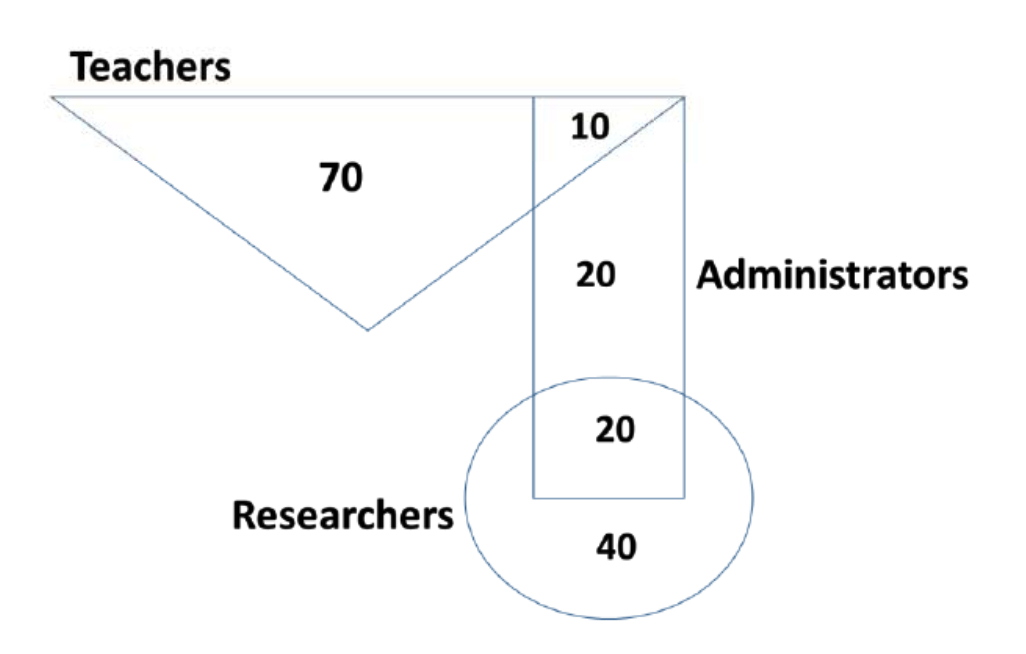
\includegraphics[width=0.5\columnwidth]{Fig/7i.png}
    \caption{}
    \label{fig:7i}
\end{figure}

\begin{multicols}{4}
    \begin{enumerate}
        \item $0$ to $15$
        \item $16$ to $30$
        \item $31$ to $45$
        \item $46$ to $60$
    \end{enumerate}
\end{multicols}

    \item "A recent High Court judgment has sought to dispel the idea of begging as a disease which leads to its stigmatization and criminalization and to regard it as a symptom. The underlying disease is the failure of the state to protect citizens who fall through the social security net."

Which one of the following statements can be inferred from the given passage?

\hfill{\brak{\text{GATE CH 2019}}}
    \begin{enumerate}
        \item Beggars are lazy people who beg because they are unwilling to work
        \item Beggars are created because of the lack of social welfare schemes
        \item Begging is an offence that has to be dealt with firmly
        \item Begging has to be banned because it adversely affects the welfare of the state
    \end{enumerate}
    
    \item In a college, there are three student clubs. Sixty students are only in the Drama club, $80$ students are only in the Dance club, $30$ students are only in the Maths club, $40$ students are in both Drama and Dance clubs, $12$ students are in both Dance and Maths clubs, $7$ students are in both Drama and Maths clubs, and $2$ students are in all the clubs. If $75$\% of the students in the college are not in any of these clubs, then the total number of students in the college is \rule{1cm}{0.1mm}.
    
\hfill{\brak{\text{GATE CH 2019}}}
\begin{multicols}{4}
    \begin{enumerate}
        \item $1000$
        \item $975$
        \item $900$
        \item $225$
    \end{enumerate}
\end{multicols}
\newpage
    \item Three of the five students allocated to a hostel put in special requests to the warden. Given the floor plan of the vacant rooms, select the allocation plan that will accommodate all their requests.
   
\begin{enumerate}[label = ]
    \item Request by X. Due to pollen allergy, I want to avoid a wing next to the garden. 

    \item Request by Y: I want to live as far from the washrooms as possible, since I am very sensitive to smell.

    \item Request by Z: I believe in Vaastu and so want to stay in the South-west wing
\end{enumerate}

The shaded rooms are already occupied. WR is washroom.

 \hfill{\brak{\text{GATE CH 2019}}}
\begin{figure}[H]
    \centering
    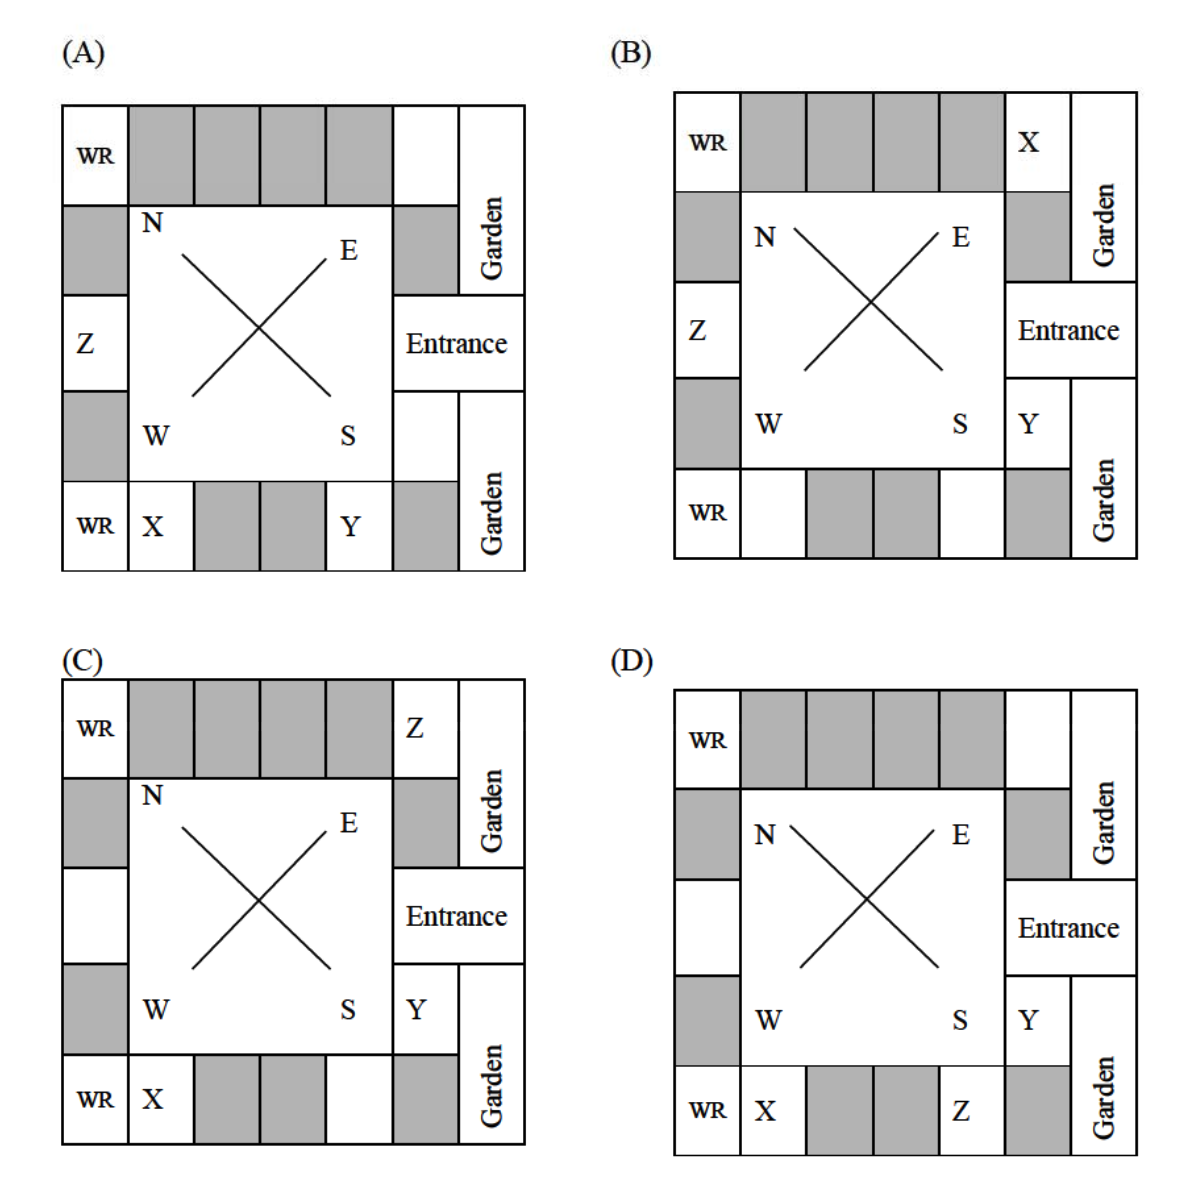
\includegraphics[width=0.9\columnwidth]{Fig/10i.png}
    \caption{}
    \label{fig:10i}
\end{figure}
\end{enumerate}
\begin{center}
    \subsection*{END OF QUESTION PAPER}
\end{center}
\newpage

\begin{enumerate}
    \item A system of $n$ homogeneous linear equations containing $n$ unknowns will have non-trivial solutions if and only if the determinant of the coefficient matrix is
    
 \hfill{\brak{\text{GATE CH 2019}}}
\begin{multicols}{4}
    \begin{enumerate}
        \item $1$
        \item $-1$
        \item $0$
        \item $\infty$
    \end{enumerate}
\end{multicols}

    \item The value of the expression $\lim_{x\to\frac{\pi}{2}}\big|\frac{tan x}{x}\big|$  is
    
 \hfill{\brak{\text{GATE CH 2019}}}
\begin{multicols}{4}
    \begin{enumerate}
        \item $\infty$
        \item $0$
        \item $1$
        \item $-1$
    \end{enumerate}
\end{multicols}
    \item Consider a rigid, perfectly insulated, container partitioned into two unequal parts by a thin membrane (see figure). One part contains one mole of an ideal gas at pressure {$P_i$} and temperature $T_i$ while the other part is evacuated. The membrane ruptures, the gas fills the entire volume and the equilibrium pressure is $P_f = P_i/4$. If $C_p$(molar specific heat capacity at constant pressure),$C_p$(molar specific heat capacity at constant volume) and R(universal gas constant) have the same units as molar entropy, the change in molar entropy $\brak{S_f - S_i}$ is
    
 \hfill{\brak{\text{GATE CH 2019}}}
 \begin{figure}[H]
     \centering
     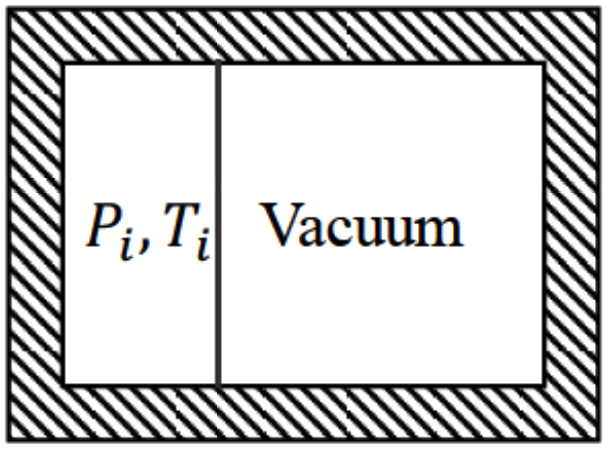
\includegraphics[width=0.3\columnwidth]{Fig/3.png}
     \caption{}
     \label{fig:3}
 \end{figure}

    \begin{enumerate}
        \item $C_p\ln{2} + R\ln{4}$
        \item -$C_p \ln{2} + R\ln{4}$
        \item R$\ln{4}$
        \item $C_p \ln{2}$
    \end{enumerate}

    

    \item For a single component system, vapor (subscript $g$) and liquid (subscript $f$) coexist in mechanical, thermal and phase equilibrium when 
    
 \hfill{\brak{\text{GATE CH 2019}}}
\begin{enumerate}
    \item $u_g = u_f$ (equality of specific internal energy)
    \item $h_g = h_f$ (equality of specific enthalpy)
    \item $s_g = s_f$ (equality of specific entropy)
    \item $g_g = g_f$ (equality of specific Gibbs free energy)
\end{enumerate}

    \item  For a binary nonideal A-B mixture exhibiting a minimum boiling azeotrope, the activity coefficients, $\gamma_i\brak{i = A,B}$, must satisfy
    
 \hfill{\brak{\text{GATE CH 2019}}}
\begin{enumerate}
    \item $\gamma_A > 1$, $\gamma_B > 1$
    \item $\gamma_A < 1$, $\gamma_B > 1$
    \item $\gamma_A = 1$, $\gamma_B = 1$
    \item $\gamma_A < 1$, $\gamma_B < 1$
\end{enumerate}

    \item For a fully-developed turbulent hydrodynamic boundary layer for flow past a flat plate, the thickness of the boundary layer increases with distance $x$ from the leading edge of the plate, along the free-stream flow direction, as
    
     \hfill{\brak{\text{GATE CH 2019}}}
\begin{multicols}{4}
    \begin{enumerate}
        \item $x^{0.5}$
        \item $x^{1.5}$
        \item $x^{0.4}$
        \item $x^{0.8}$
    \end{enumerate}
\end{multicols}

    \item Consider a cylinder (dimeter D and length D), a sphere (dimeter D) and a cube (side length D). Which of the following statements concerning the sphericity($\Phi$) of the above objects is true:
    
     \hfill{\brak{\text{GATE CH 2019}}}
\begin{multicols}{2}
    \begin{enumerate}
        \item $\phi_{sphere} > \phi_{cylinder} > \phi_{cube}$
        \item $\phi_{sphere} = \phi_{cylinder} = \phi_{cube}$
        \item $\phi_{sphere} < \phi_{cylinder} < \phi_{cube}$
        \item $\phi_{sphere} > \phi_{cylinder} = \phi_{cube} $
    \end{enumerate}
\end{multicols}

    \item Prandtl number signifies the ratio of
    
     \hfill{\brak{\text{GATE CH 2019}}}
\begin{multicols}{2}
    \begin{enumerate}
    \item $\frac{Momentum diffusivity}{Thermal Diffusivity}$
    \item $\frac{Mass Diffusivity}{Thermal Diffusivity}$
    \item $\frac{Thermal Diffusivity}{Momentum diffusivity}$
    \item $\frac{Thermal Diffusivity}{Mass diffusivity}$
    \end{enumerate}
\end{multicols}

    \item Pool boiling equipment operating above ambient temperature is usually designed to operate
    
     \hfill{\brak{\text{GATE CH 2019}}}
\begin{multicols}{2}
    \begin{enumerate}
        \item far above the critical heat flux
        \item near the critical heat flux
        \item far above the Leidenfrost point
        \item near the Leidenfrost point
    \end{enumerate}
\end{multicols}
\newpage

    \item  The desired liquid-phase reaction

    

     $D + E \overset{k_1}{\to} F \hspace{8pt} r_F = k_1 {C_D}^{2} {C_E}^{0.3}$ 

   
    \text{is accompanies by an undesired side reaction} 
        
            $D + E \overset{k_2}{\to} G \hspace{8pt} r_G = k_2 {C_D}^{0.4} {C_E}^{1.5}$
    
        
Four isothermal reactor schemes (CSTR: ideal Continuous-Stirred Tank Reactor; PFR: ideal Plug Flow Reactor) for processing equal molar feed rates of D and E are shown in the figure. Each scheme is designed for the same conversion. The scheme that gives the most favorable product distribution is:

 \hfill{\brak{\text{GATE CH 2019}}}
\begin{figure}[H]
    \centering
    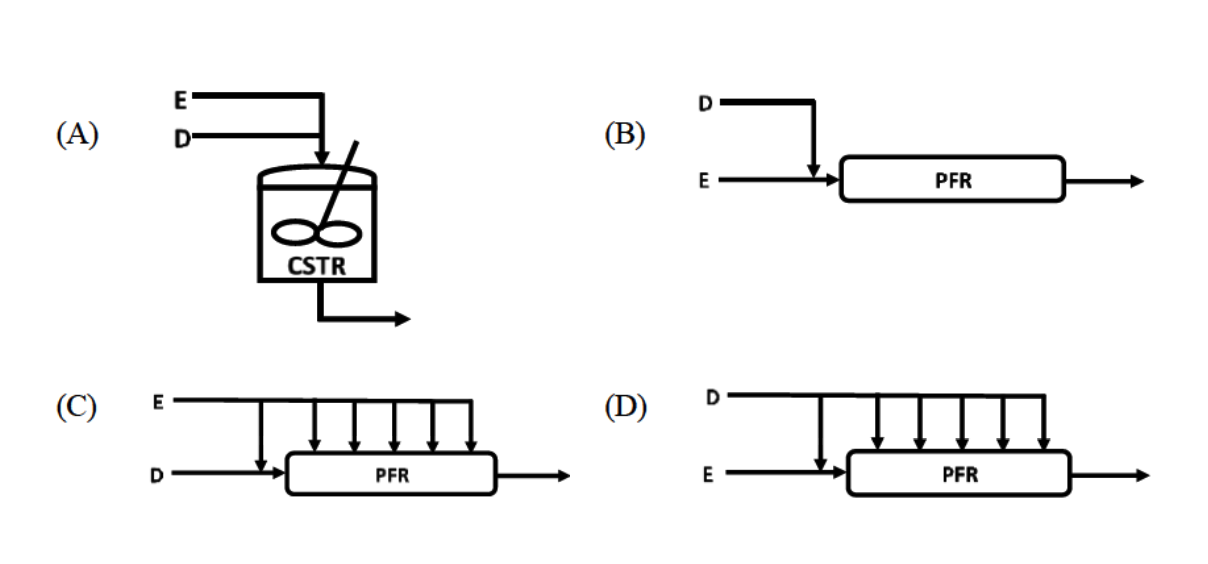
\includegraphics[width=1\columnwidth]{Fig/10.png}
    \caption{}
    \label{fig:10}
\end{figure}

    \item For a first order reaction in a porous spherical catalyst pellet, diffusional effects are the most likely to lower the observed rate of reaction for
    
 \hfill{\brak{\text{GATE CH 2019}}}
\begin{enumerate}
    \item slow reaction in a pellet of small diameter
    \item slow reaction in a pellet of large diameter
    \item fast reaction in a pellet of small diameter
    \item fast reaction in a pellet of large diameter
\end{enumerate}

      \item  A thermocouple senses temperature based on the 
      
 \hfill{\brak{\text{GATE CH 2019}}}
  

\begin{multicols}{4}
    \begin{enumerate}
        \item Nernst Effect
        \item Maxwell Effect
        \item Seebeck Effect
        \item Peltier Effect
    \end{enumerate}
\end{multicols}

    \item The correct expression for the Colburn $j$-factor for mass transfer that relates Sherwood number(Sh), Reynolds number(Re) and Schmidt number(Sc) is
    
 \hfill{\brak{\text{GATE CH 2019}}}
\begin{multicols}{4}
    \begin{enumerate}
        \item $\frac{Sh}{\brak{Re}\brak{Sc}^{1/3}}$
        \item $\frac{Sh}{\brak{Re}^{1/2}\brak{Sc}}$
        \item $\frac{Sh}{\brak{Re}^{1/2}\brak{Sc}^{1/3}}$
        \item $\frac{Sh}{\brak{Re}\brak{Sc}}$
    \end{enumerate}
\end{multicols}

    \item In the drying of non-dissolving solids at constant drying conditions, the internal movement of moisture in the solid has a dominant effect on the drying rate during
    
     \hfill{\brak{\text{GATE CH 2019}}}
\begin{enumerate}
    \item the initial adjustment period only
    \item the constant rate period only
    \item the falling rate period only
    \item both the initial adjustment and constant rate periods
\end{enumerate}

    \item Three distillation schemes for separating an equimolar, constant relative volatility ABC mixture into nearly pure components are shown. The usual simplifying assumptions such as constant molal overflow, negligible heat loss, ideal trays are valid. All the schemes are designed for minimum total reboiler duty. Given that the relative volatilities are in the ratio $\alpha_A:\alpha_B:\alpha_C \equiv$ 8:2:1, the correct option that arranges the optimally-designed schemes in ascending order of total reboiler duty is
    
     \hfill{\brak{\text{GATE CH 2019}}}
     \begin{figure}[H]
         \centering
         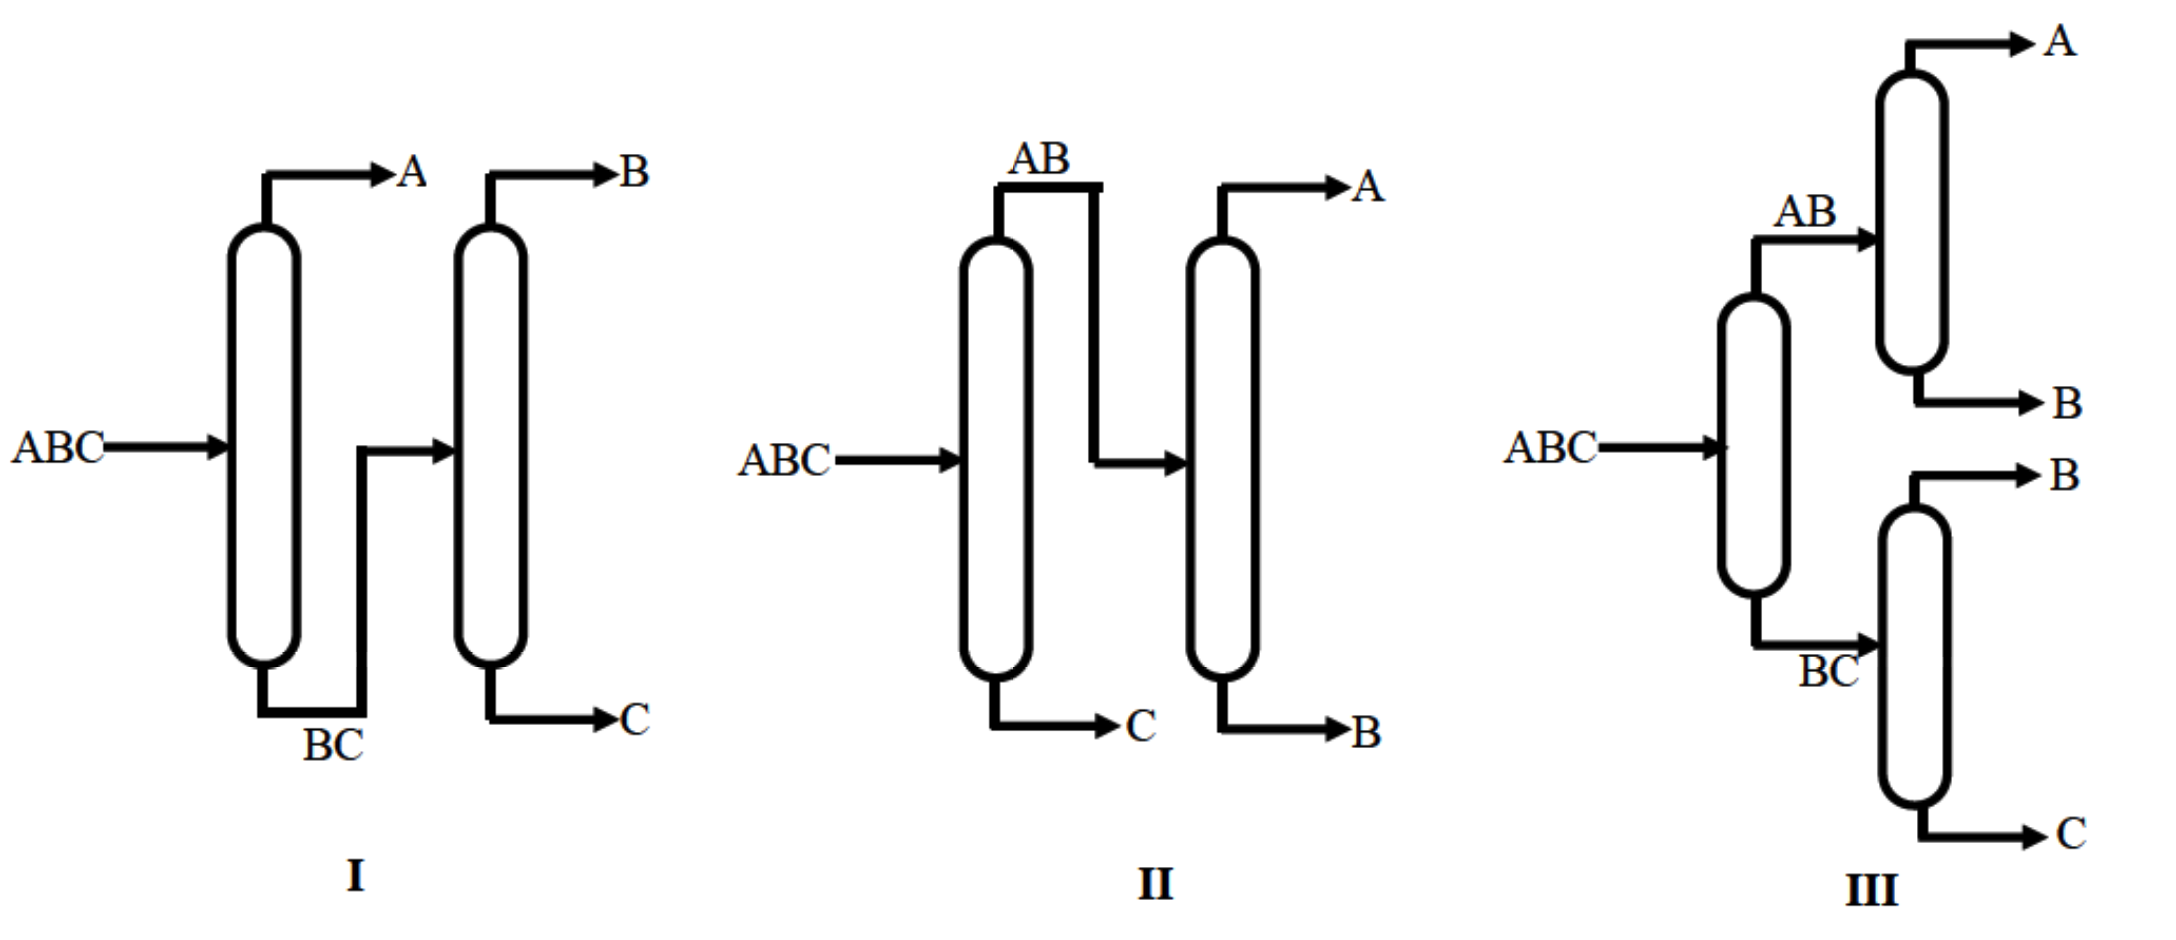
\includegraphics[width=0.85\columnwidth]{Fig/15.png}
         \caption{}
         \label{fig:15}
     \end{figure}

\begin{multicols}{4}
    \begin{enumerate}
        \item I,II,III
        \item III,I,II
        \item II,I,III
        \item III,II,I
    \end{enumerate}
\end{multicols}
\newpage
    \item Consider the two countercurrent heat exchanger designs for heating a cold stream from $t_in$ to $t_out$ as shown in figure. The hot process stream available at $T_in$ The inlet stream conditions and overall hest transfer coefficients are identical in both the designs. The heat transfer area in Design I and Design II are respectively $A^{I}_{HX}$ and $A^{II}_{HX}$ 
\begin{figure}[H]
    \centering
    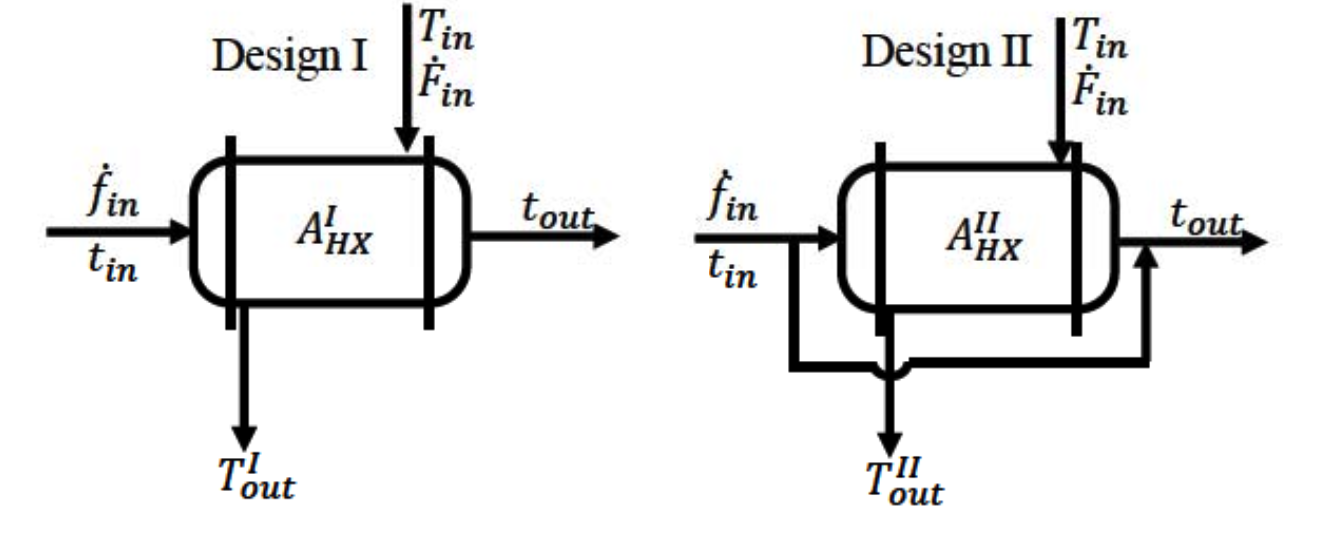
\includegraphics[width=0.5\columnwidth]{Fig/16.png}
    \caption{}
    \label{fig:16}
\end{figure}
    If heat losses are neglected, and if both the designs are feasible, which of the following statements holds true:
    
    \hfill{\brak{\text{GATE CH 2019}}}
\begin{enumerate}
     \item $A^{I}_{HX} > A^{II}_{HX}$ \hspace{5pt} $T^{I}_{out} > T^{II}_{out}$
    \item $A^{I}_{HX} = A^{II}_{HX}$ \hspace{5pt}  $T^{I}_{out} = T^{II}_{out}$
    \item $A^{I}_{HX} < A^{II}_{HX}$ \hspace{5pt}  $T^{I}_{out} > T^{II}_{out}$
    \item $A^{I}_{HX} < A^{II}_{HX}$  \hspace{5pt}  $T^{I}_{out} = T^{II}_{out}$
\end{enumerate} 

    \item Producer gas is obtained by
    
 \hfill{\brak{\text{GATE CH 2019}}}
 
\begin{enumerate}
    \item passing air through red hote coke
    \item thermal cracking of naphtha
    \item passing steam through red hot coke
    \item passing air and steam through red hot coke
\end{enumerate}
    \item In Kraft process, the essential chemical reagents used in the digester are    
    
 \hfill{\brak{\text{GATE CH 2019}}}
 
\begin{enumerate}
    \item caustic soda, mercaptans and ethylene oxide
    \item caustic soda, sodium sulphide and soda ash
    \item quick lime, salt cake and dimethyl sulphide
    \item baking soda, sodium sulphide and mercaptans
\end{enumerate}

    \item
        The most common catalyst used for oxidation of 0-xylene to pthalic anhydride is
        
  \hfill{\brak{\text{GATE CH 2019}}}
\begin{enumerate}
    \item $V_2 O_5$
    \item Pd
    \item Pt
    \item Ag
\end{enumerate}

    \item In petroleum refining operations, the process used for converting paraffins and naphthenes to aromatics is
    
 \hfill{\brak{\text{GATE CH 2019}}}
 
\begin{enumerate}
    \item alkylation
    \item catalytic reforming
    \item hydrocracking
    \item isomerization
\end{enumerate}


    \item The combination that correctly matches the polymer in Group-1 with the polymerization reaction type in Group-2 is
    
 \hfill{\brak{\text{GATE CH 2019}}}
 
\begin{multicols}{2}
    \textbf{Group1}
    \begin{enumerate}[label=(\Alph*)]
        \item Nylon 6
        \item Polypropylene
        \item Polyester
    \end{enumerate}
\columnbreak

    \textbf{Group-2}
    \begin{enumerate}[label=(\Roman*)]
        \item Condensation
        \item Ring opening polymerization
        \item Addition polymerization
    \end{enumerate}
\end{multicols}
\begin{multicols}{2}
    \begin{enumerate}
        \item A-II, B-I, C-III
        \item A-I, B-III, C-II
        \item A-III, B-II, C-I
        \item A-II, B-III, C-I
    \end{enumerate}
\end{multicols}

    \item 
        The product of the eigenvalues of the matrix  $\myvec{
            2 & 3 \\
            0 & 7
        }$ is \rule{2cm}{0.1mm} (rounded off to one decimal place).
        
  \hfill{\brak{\text{GATE CH 2019}}}    

    \item For a hydraulic lift with dimensions shown in figure, assuming g = $10$ m/$s^2$, the maximum diameter $D_left$(in m) that lifts a vehicle of mass $1000$ kg using a force of $100$ N is (rounded off to two decimal places).
    
 \hfill{\brak{\text{GATE CH 2019}}}
    \begin{figure}[H]
        \centering
        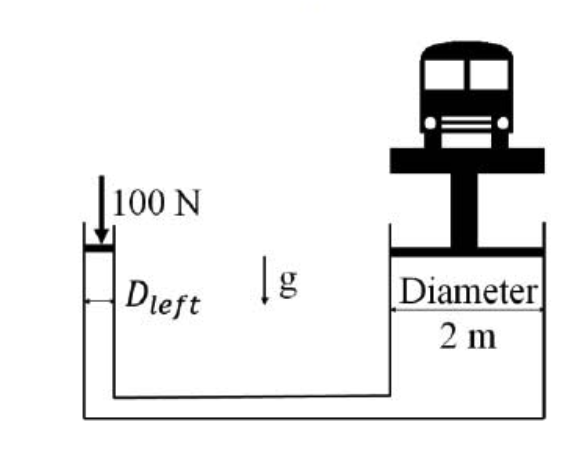
\includegraphics[width=0.4\columnwidth]{Fig/23.png}
        \caption*{}
        \label{fig: 23}
    \end{figure}

\item The liquid flow rate through an equal percentage control valve, when fully open, is $150$ gal/min and the corresponding pressure drop is $50$ psi. If the specific gravity of the liquid is $0.8$, then the valve coefficient, $C_v$, in gal/(min $psi^{0.5}$) is  \rule{1cm}{0.1mm} (rounded off to two decimal places).

 \hfill{\brak{\text{GATE CH 2019}}}
    \item Consider a sealed rigid bottle containing $CO_2$ and $H_2$O at $10$ bar and ambient temperature. Assume that the gas phase in the bottle is pure $CO_2$ and follows the ideal gas law. The liquid phase in the bottle contains $CO_2$ dissolved in $H_2$O and is an ideal solution. The Henry's constant at the system pressure and temperature is $H_CO_2 = 1000$ bar. The equilibrium mole :fraction of $CO_2$ dissolved in $H_2$O is \rule{1cm}{0.1mm} (rounded off to three decimal places).   
    
 \hfill{\brak{\text{GATE CH 2019}}}
    \item 
        The solution of the ordinary differential equation $\frac{dy}{dx} + 3y = 1$, subject to the initial condition $y = 1$ at $x = 0$ , is 
        
      \hfill{\brak{\text{GATE CH 2019}}}
    
\begin{multicols}{2}
    \begin{enumerate}
        \item $\frac{1}{3}\brak{1 + 2e^{-x/3}}$
        \item $\frac{1}{3}\brak{5 - 2e^{-x/3}}$
        \item $\frac{1}{3}\brak{5 - 2e^{-3x}}$
        \item $\frac{1}{3}\brak{1 + 2e^{-3x}}$
    \end{enumerate}
\end{multicols}

    \item 
        the value of the complex number ${i}^{-1/2}$(where ${i} = \sqrt{-1}$) is
        
     \hfill{\brak{\text{GATE CH 2019}}}

\begin{multicols}{4}
    \begin{enumerate}
    
    \item $\frac{1}{\sqrt{2}}\brak{1 -i}$
    \item $-\frac{1}{\sqrt{2}}i$
    \item $\frac{1}{\sqrt{2}}i$
    \item $\frac{1}{\sqrt{2}}\brak{1+i}$
    \end{enumerate}
\end{multicols}

    \item An incompressible Newtonian fluid flows in a pipe of diameter $D_1$ at volumetric flow rate Q. Fluid with same properties flows in another pipe of diameter $D2 = D1 / 2$ at the same flow rate Q. The transition length required for achieving fully-developed flow is $l_1$ for the tube of diameter $D_1$ , while it is $l_2$ for the tube of diameter $D_2$.Assuming steady laminar flow in both cases, the ratio $l_1/l_2$ is: 
    
     \hfill{\brak{\text{GATE CH 2019}}}
    \begin{multicols}{4}
\begin{enumerate}
    \item $1/4$
    \item $1$
    \item $2$
    \item $4$
\end{enumerate}
\end{multicols}

    \item A disk turbine is used to stir a liquid in a baffled tank. To design the agitator, experiments are performed in a lab-scale model with a turbine diameter of $0.05$ m and a turbine impeller speed of $600$ rpm. The liquid viscosity is $0.001$ Pa s while the liquid density is $1000 kg/m^3$ . The actual application has a turbine diameter of $0.5$ m, an impeller speed of $600$rpm, a liquid viscosity of $0.1$Pa s and a liquid density of $1000 kg/m^3$ . The effect of gravity is negligible. If the power required in the lab-scale model is $P_1$; and the estimated power for the actual application is $P_2$ , then the ratio $P_1/P_2$ is 
    
     \hfill{\brak{\text{GATE CH 2019}}}
\begin{multicols}{4}
    \begin{enumerate}
        \item $10^3$
        \item $10^4$
        \item $10^5$
        \item $10^6$
        \end{enumerate}
\end{multicols}
\newpage
    \item 
        Consider two non-interacting tanks-in-series as shown in figure. Water enters TANK 1 at $q cm^3/s$ and drains down to TANK 2 by gravity at a rate $k\sqrt{h_1}\brak{cm^3/s}$. Similarly, water drains from TANK 2 by gravity at a rate of $k\sqrt{h_2}\brak{cm^3/s}$ where $h_1$ and $h_2$ represent levels of TANK 1 and TANK 2, respectively (see figure). Drain valve constant $k = 4 cm^{2.5}/s$ and cross sectional areas of the two tanks are $A_1 = A_2 = 28 cm^2$.
     

\begin{figure}[H]
    \centering
    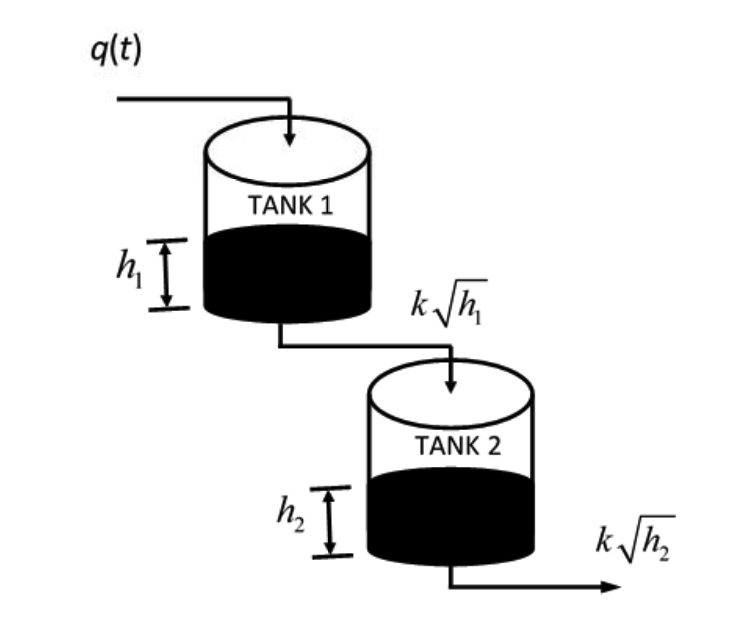
\includegraphics[width=0.4\columnwidth]{Fig/30.png}
    \caption*{}
    \label{fig: 30}
  
\end{figure}

       At steady state operation, the water inlet flow rate is $q_{ss} = 16 cm^3/s$. The transfer function relating the deviation variables $\tilde{h_2}\brak{cm}$ to flow rate $\tilde{q}\brak{cm^3/s}$ is,
       
\hfill{\brak{\text{GATE CH 2019}}}
 

\begin{multicols}{4}
    \begin{enumerate}
        \item $\frac{2}{\brak{56s + 1}^{2}}$
        \item $\frac{2}{\brak{62s + 1}^{2}}$
        \item $\frac{2}{\brak{36s + 1}^{2}}$
        \item $\frac{2}{\brak{49s + 1}^{2}}$
    \end{enumerate}
\end{multicols}
\newpage
    \item 
         Choose the option that correctly matches the step response curves on the left with the appropriate transfer functions on the right. The step input change occurs at time $t=O$. 
         
    \hfill{\brak{\text{GATE CH 2019}}}
\begin{figure}[H]
  \centering
    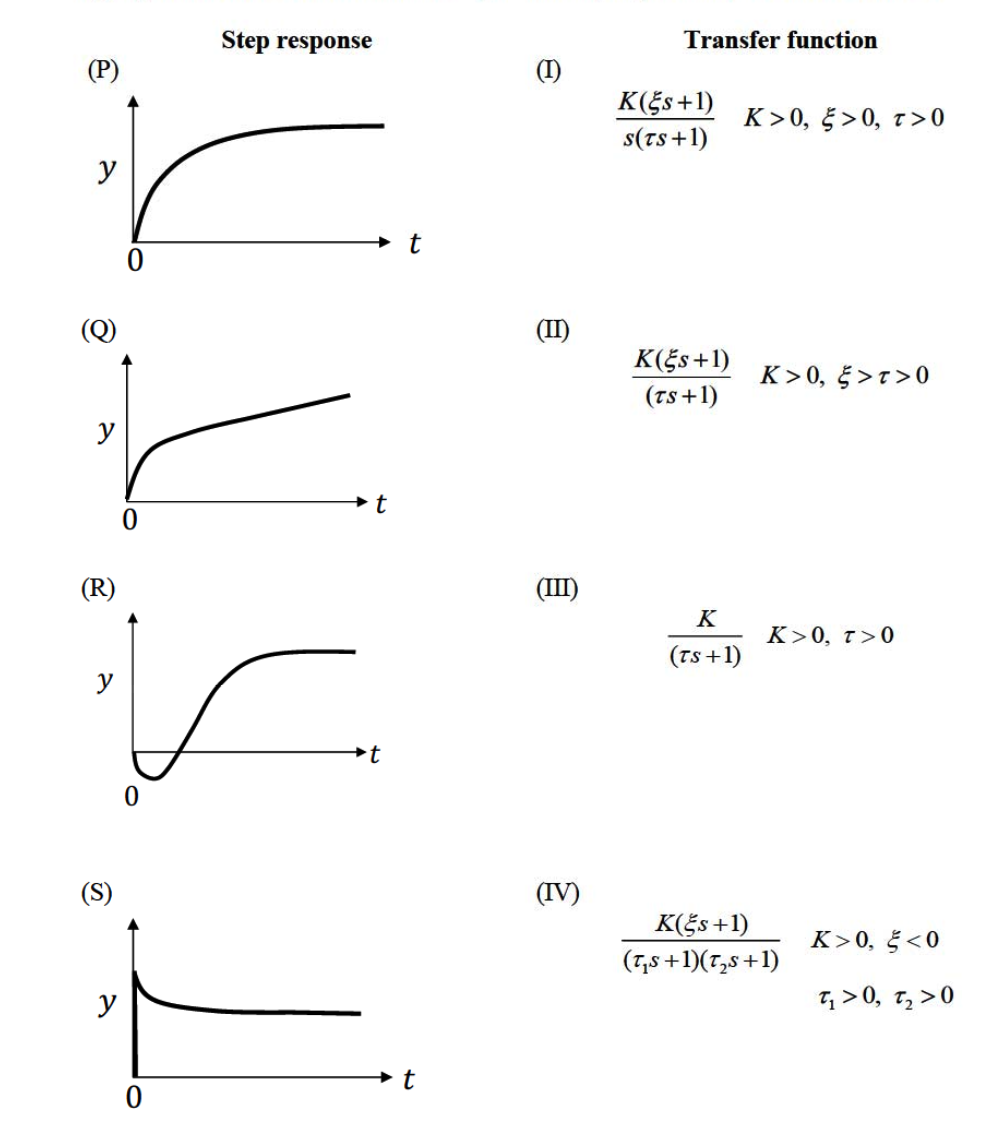
\includegraphics[width=0.8\columnwidth]{Fig/34.png}
   \caption*{}
    \label{fig: 31}
\end{figure}
\begin{multicols}{2}
    \begin{enumerate}
        \item A-III, B-IV, C-II, D-I
        \item A-III, B-I, C-IV, D-II
        \item A-IV, B-III, C-II, D-I
        \item A-III, B-II, C-IV, D-I
    \end{enumerate}
\end{multicols}
\newpage
    \item 
         100 kg of a feed containing 50 wt.\% of a solute C is contacted with 80 kg of a solvent containing 0.5 wt.\% of C in a mixer-settler unit. From this operation, the resultant extract and raffinate phases contain 40 wt.\% and 20 wt.\% of C, respectively. If E and R denote the mass of the extract and raffinate phases, respectively, the ratio E/R is 
        
\hfill{\brak{\text{GATE CH 2019}}}
    
\begin{multicols}{4}
    \begin{enumerate}
        \item $1/4$
        \item $1/2$
        \item $2/3$
        \item $1$
    \end{enumerate}
\end{multicols}

    \item 
         The combination that correctly matches the process in Group-1 with the entries in Group-2 is
    
    \hfill{\brak{\text{GATE CH 2019}}}

\begin{multicols}{2}
    \begin{enumerate}[label = \Alph*)]
        \item Wulff process
        \item Sulfite process
        \item Solvay Process
        \item Frasch process
    \end{enumerate}
\columnbreak
    \begin{enumerate}[label = \Roman*)]
        \item Sulfur mining
        \item Sods ash production 
        \item Acetylene prodcution
        \item Pulp production
    \end{enumerate}
\end{multicols}
\begin{multicols}{2}
    \begin{enumerate}
        \item A-II, B-IV, C-III, D-I
        \item A-III, B-IV, C-II, D-I
        \item A-IV, B-I, C-II, D-III
        \item A-II, B-I, C-IV, D-III
    \end{enumerate}
\end{multicols}

    \item If x,y and z are directions in a Cartesian coordinate system and i,j and k are the respective unit vectors, the directional derivative of the function $u\brak{x,y,z} = x^2 - 3yz$ at the point $\brak{2, 0,-4}$ in the direction $\brak{i+j-2k}/\sqrt{6}$ is \rule{2cm}{0.1mm} (rounded off to two decimal places).
    
\hfill{\brak{\text{GATE CH 2019}}}
    \item Two unbiased dice are thrown. Each dice can show any number between $1$ and $6$. The probability that the sum of the outcomes of the two dice is divisible by $4$ is \rule{1cm}{0.1mm}(rounded off to two decimal places).
    
\hfill{\brak{\text{GATE CH 2019}}}
    \item The Newton-Raphson method is used to determine the root of the equation $f\brak{x} = e^{-x} - x$. If the initial guess for the root is $0$, the estimate of the root after two iterations is (rounded off to three decimal places). 
    
\hfill{\brak{\text{GATE CH 2019}}}
    \item Carbon monoxide (CO) reacts with hydrogen sulphide ($H_2S$) at a constant temperature of $800$ K and a constant pressure of $2$ bar as: 
    \begin{align*}
        CO + H_2S \rightleftharpoons COS + H_2
    \end{align*}
    The Gibbs free energy of the reaction $\Delta g^{o}_{rxn} = 22972.3$ J/mol and universal gas constant $R = 8.314$ J/(mol K). Both the reactants and products can be assumed to be ideal gases. If initially only $4$ mol of $H_2S$ and $1$ mol of CO are present, the extent of the reaction (in mol) at equilibrium is \rule{1.5cm}{0.1mm}(rounded off to two decimal places).
    
\hfill{\brak{\text{GATE CH 2019}}}
    \item For a given binary system at constant temperature and pressure, the molar volume (in $m^3/mol$) is given by: $v = 30x_A + 20x_B + x_Ax_B\brak{15x_A - 7x_B}$ , where $x_A $and $x_B$ are the mole fractions of components A and B, respectively. The volume change of mixing $\Delta v_{mix}$ (in $m^3/mol$) at $x_A = 0.5$ is \rule{1.5cm}{0.1mm}(rounded off to one decimal place). 
    
\hfill{\brak{\text{GATE CH 2019}}}
\newpage
    \item Consider a vessel containing steam at $180^oC$ The initial steam quality is $0.5$ and the initial volume of the vessel is $1 m^3$ . The vessel loses heat at a constant rate q under isobaric conditions so that the quality of steam reduces to $0.1$ after $10$ hours. The thermodynamic properties of water at $180^oC$ are (subscript g: vapor phase; subscript f : liquid phase): 
    
    \begin{align*}
        \text{specific volume:} & v_g = 0.19405 m^3/kg,  v_f = 0.001127 m^3/kg; \\
        \text{specific internal energy:} & u_g = 2583.7 kJ/Kg,  u_f = 762.08 kJ/Kg;\\
        \text{specific enthalpy:} & h_g = 2778.3 kJ/Kg,  h_f = 763.21 kJ/Kg.
    \end{align*} 
    The rate of heat loss q (in kJ/hour) is \rule{2cm}{0.1mm}(rounded off to the nearest integer).
    
\hfill{\brak{\text{GATE CH 2019}}}
    \item A fractionator recovers 95 mol \% n-propane as the distillate from an equimolar mixture of n-propane and n-butane. The condensate is a saturated liquid at 55 °C. The Antoine equation is of the form, $\ln\brak{P^{sat}\sbrak{in bar}} = A - \frac{B}{T\sbrak{in K} + C}$, and the constants are provided below: 

    \begin{table}[h!]
\centering
\begin{tabular}{|c|c|c|c|}
    \hline
     & A & B & C \\
    \hline
    n-propane & 9.1058 & 1872.46  & - 25.16  \\
    \hline
    n- butane & 9.0580 & 2154.90 & -34.42 \\
    \hline
\end{tabular}    
\end{table}

    Assuming Raoult's law, the condenser pressure (in bar) is \rule{3cm}{0.1mm} (rounded off to one decimal place).
    
\hfill{\brak{\text{GATE CH 2019}}}
    \item A centrifugal pump is used to pump water (density $1000 kg/m^3$ ) from an inlet pressure of $10^5$ Pa to an exit pressure of $2*10^5$ Pa. The exit is at an elevation of 10 m above the pump. The average velocity of the fluid is 10 m/s. The cross-sectional area of the pipes at the pump inlet and outlet is $10^{-3} m^2$ and acceleration due to gravity is $g = 10 m/s^2 $. Neglecting losses in the system, the power (in Watts) delivered by the pump is \rule{1.5cm}{0.1mm}(rounded off to the nearest integer). 
    
\hfill{\brak{\text{GATE CH 2019}}}
    \item A solid sphere of radius 1 cm and initial temperature of $25^oC$ is exposed to a gas stream at $100^oC$. For the solid sphere, the density is $104 kg/m^3$ and the specific heat capacity is $500 J/(kg K)$. The density of the gas is $0.6 kg/m^3$ and its specific heat capacity is $10^3 J/(kg K)$. The solid sphere is approximated as a lumped system $\brak{Biot number \ll 1}$ and all specific heats are constant. If the heat transfer coefficient between the solid and gas is $50 W/(m^2 K)$, the time (in seconds) needed for the sphere to reach $95^oC$ is \rule{2cm}{0.1mm} (rounded off to the nearest integer).
    
\hfill{\brak{\text{GATE CH 2019}}}
    \item Stream A with specific heat capacity $C_{PA}= 2000 J/(kg K)$ is cooled from 90°C to 45°C in a concentric double pipe counter current heat exchanger having a heat transfer area of $8m^2$ .The cold stream B of specific heat capacity $C_{PB} = 1000 J/(kg K)$ enters the exchanger at a flow rate 1 kg/s and 40°C The overall heat transfer coefficient $U = 250 W/(m^2 K)$. Assume that the mean driving force is based on the arithmetic mean temperature difference, that is, $\sbrak{\Delta T}_{AMTD} = \brak{\frac{T_{A,in} + T_{A,out}}{2}} - \brak{\frac{T_{B,in} + T_{B,out}}{2}}$ where $T_{i,in}$ and $T_{i,out}$ refer to the temperature of the $i^{th}$ stream $\brak{i = A, B}$ at the inlet and exit, respectively. The mass flow rate of stream A (in kg/s ), is \rule{2cm}{0.1mm}(rounded off to two decimal places).
    
\hfill{\brak{\text{GATE CH 2019}}}
\newpage
    \item A 20 cm diameter cylindrical solid pellet of a nuclear fuel with density $6000 kg/m^3$ and conductivity of 300 W/(m K) generates heat by nuclear fission at a spatially uniform rate of $10^4 W /kg$. The heat from the fuel pellet is transferred to the surrounding coolant by convection such that the pellet wall temperature remains constant at $300^oC$ Neglecting the axial and azimuthal dependence, the maximum temperature (in °C) in the pellet at steady state is \rule{2cm}{0.1mm} (rounded off to the nearest integer). 
    
\hfill{\brak{\text{GATE CH 2019}}}

    \item The elementary, irreversible, liquid-phase, parallel reactions, $2A \to D$ and $2A\to U$, take place in an isothermal non-ideal reactor. The C-curve measured in a tracer experiment is shown in the figure, where $C\brak{t}$ is the concentration of the tracer in $g/m^3$ at the reactor exit at time t (in min). 

\hfill{\brak{\text{GATE CH 2019}}}
\begin{figure}[H]
    \centering
    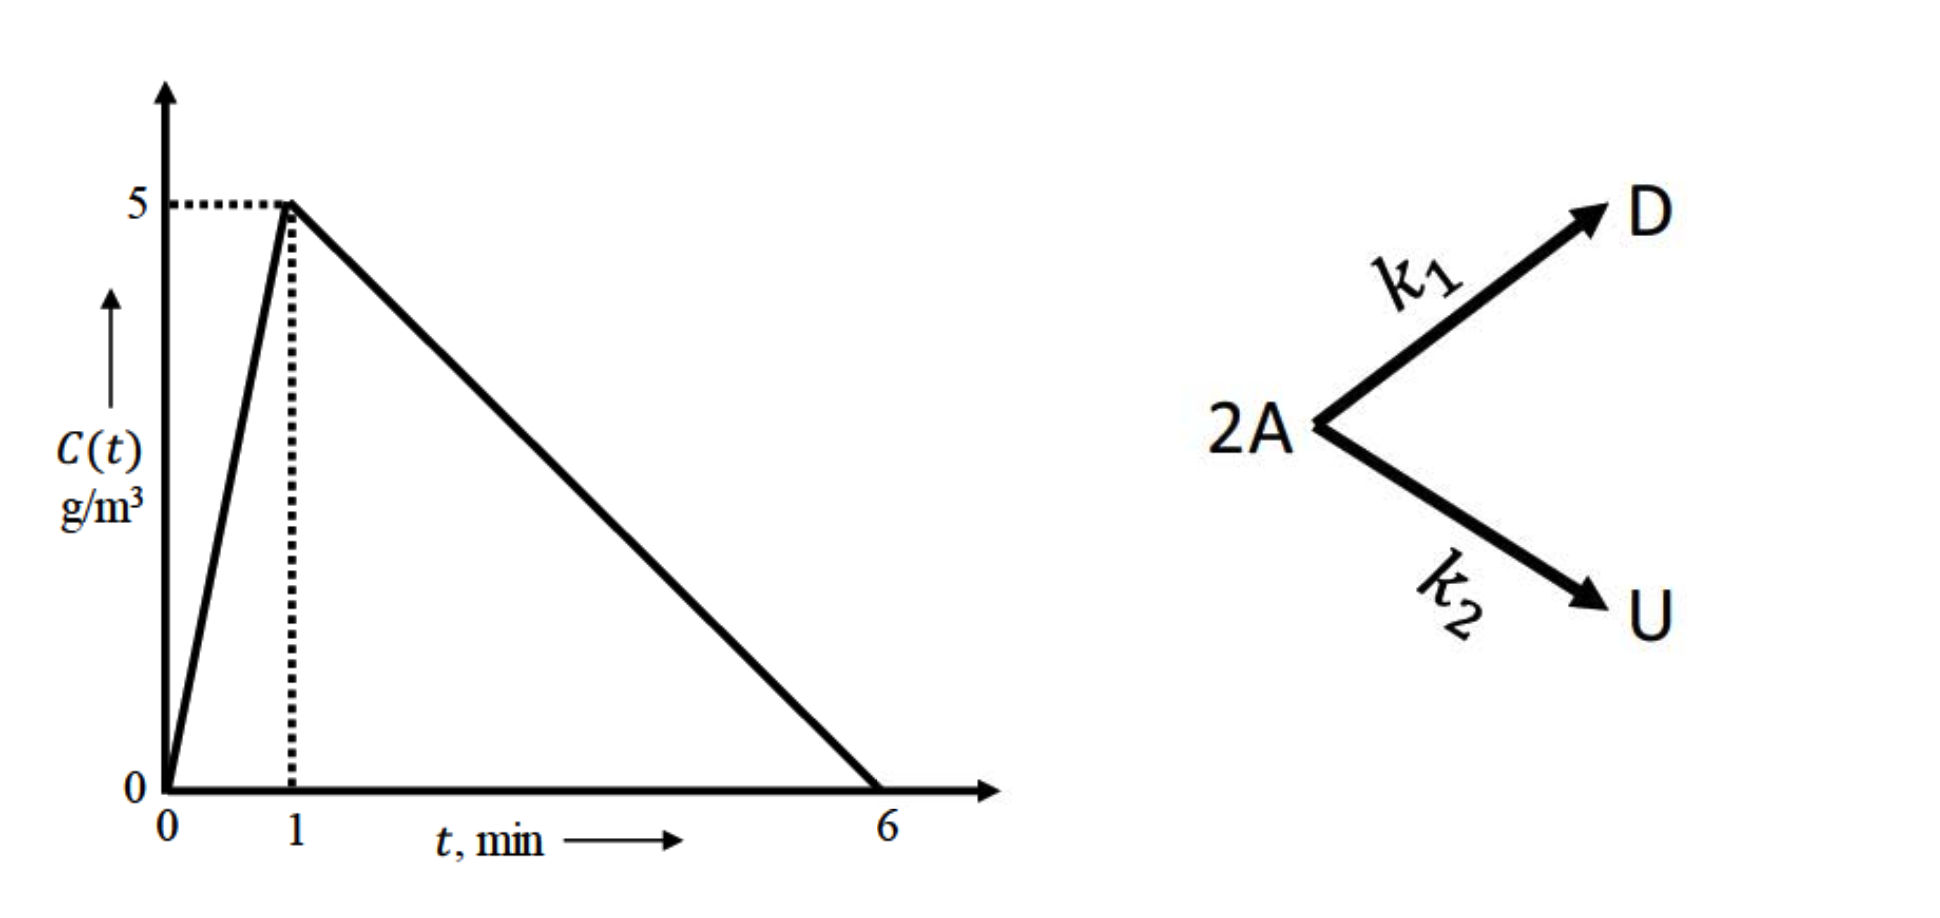
\includegraphics[width=0.9\columnwidth]{Fig/45.png}
    \caption{}
    \label{fig:45}
\end{figure}

    The rate constants are $k_1 = 0.2 Liter/(mol min)$ and $k_2 = 0.3 Liter/(mol min)$. Pure A is fed to the reactor at a concentration of 2 mol/Liter. Using the segregated model, the percentage conversion in the reactor is \rule{1.5cm}{0.1mm}(rounded off to the nearest integer).
    
\hfill{\brak{\text{GATE CH 2019}}}
\newpage
    \item A first-order irreversible liquid phase reaction $A \to B(k = 0.1 min^{-1})$ is carries out under isothermal, steady state conditions in the following reactor arrangement comprising an ideal CSTR(Continuous-Stirred Tank Reactor) and two ideal PFRs(Plug Flow Reactors). From the information in the figure, the volume of the CSTR(in Liters) is \rule{1.5cm}{0.1mm}(rounded off to the nearest integer).
    
\hfill{\brak{\text{GATE CH 2019}}}
\begin{figure}[H]
    \centering
    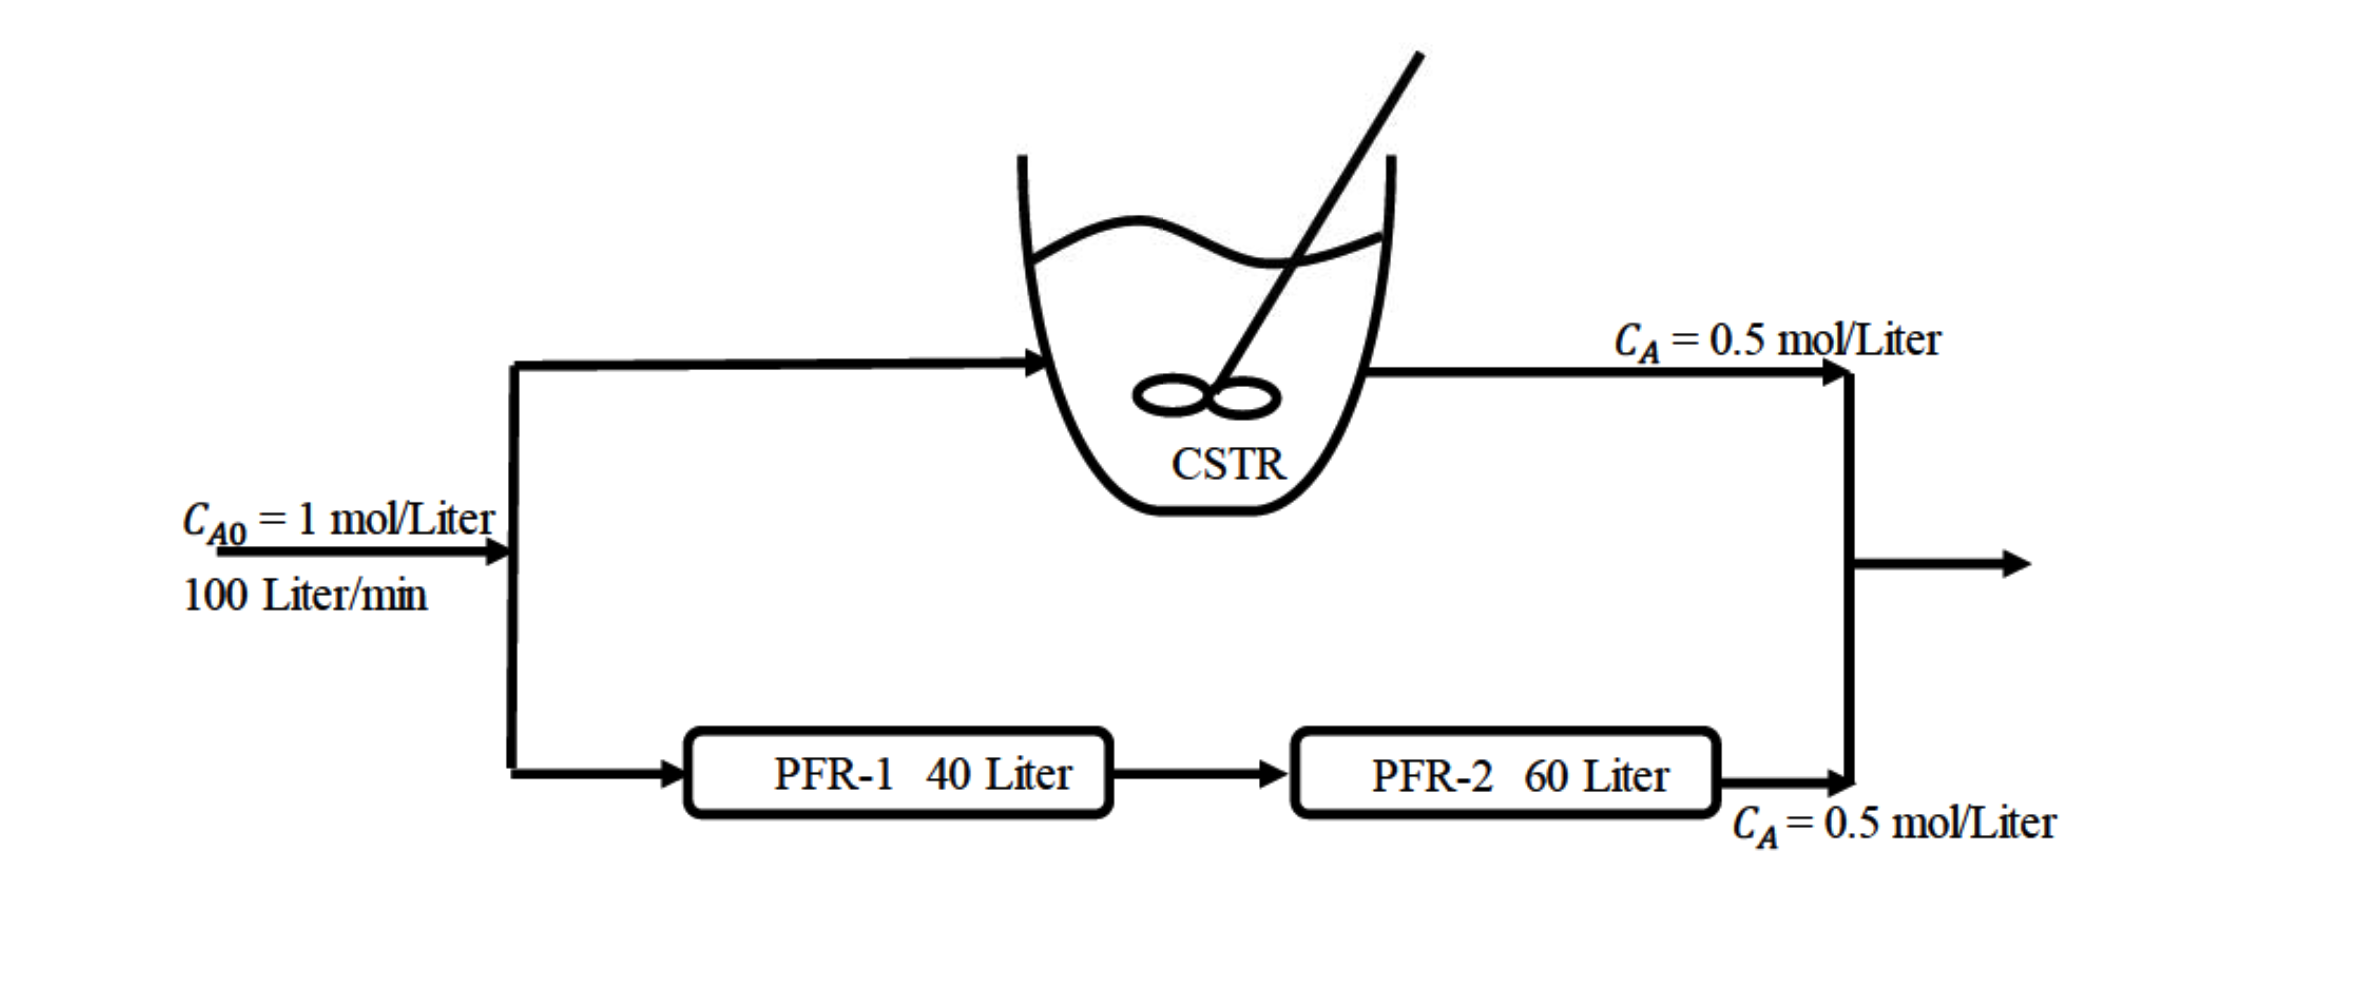
\includegraphics[width=0.6 \columnwidth]{Fig/46.png}
    \caption*{}
    \label{fig: 46}
\end{figure}
    \item 
        The elementary liquid-phase irreversible reactions 
    
\begin{align*}
     A \xrightarrow{{k_1 = 0.4 min^{-1}}} B \xrightarrow{{k_1 = 0.1 min^{-1}}} C
\end{align*}

    take place take place in an isothermal ideal CSTR (Continuous-Stirred Tank Reactor). Pure A is fed to the reactor at a concentration of 2 mol/Liter. For the residence time that maximizes the exit concentration of B, the percentage yield of B, defined as $\brak{\frac{net formation rate of B}{net formation rate of A} \times 100}$, is \rule{1.5cm}{0.1mm}(rounded off to the nearest integer).
    
\hfill{\brak{\text{GATE CH 2019}}}

    \item The elementary irreversible gas-phase reaction $A \to B + C$ is carried out adiabatically in an ideal CSTR (Continuous-Stirred Tank Reactor) operating at 10 atm. Pure A enters the CSTR at a flow rate of 10 moles and a temperature of 450 K. Assume A, B and C to be ideal gases. The specific heat capacity at constant pressure  \brak{C_{pi}} and heat of formation $\brak{H^{o}_{i}}$, of component $i \brak{i = A, B, C}$, are: 

    \begin{align*}
        C_{PA} = 30J/(mol K) \hspace{15pt} C_{PB} = 10J(mol K) \hspace{15pt} C_{PC} 20J(mol K) \\ 
        H^{o}_{A} = -90 kJ/mol \hspace{15pt} H^{o}_{B} = -54 kJ/mol \hspace{15pt} H^{o}_{C} = -45 kJ/mol 
    \end{align*}

    The reaction rate constant $k \brak{per second} = 0.133 exp^{\frac{E}{R}\brak{\frac{1}{450} - \frac{1}{T}}}$, where E = 31.4 kJ/mol and universal gas constant $R = 0.082 L atm/(mol K) = 8.314 J/(mol K)$. The shaft work may be neglected in the analysis, and specific heat capacities do not vary with temperature. All heats of formation are referenced to 273 K. The reactor volume (in Liters) for 75\% conversion is \rule{1.5cm}{0.1mm}(rounded off to the nearest integer). 
    
\hfill{\brak{\text{GATE CH 2019}}}
\newpage
    \item For the closed loop system shown in figure, the phase margin (in degrees) is \rule{2cm}{0.1mm}(rounded off to one decimal place). 
    
\hfill{\brak{\text{GATE CH 2019}}}
    \begin{figure}[H]
        \centering
        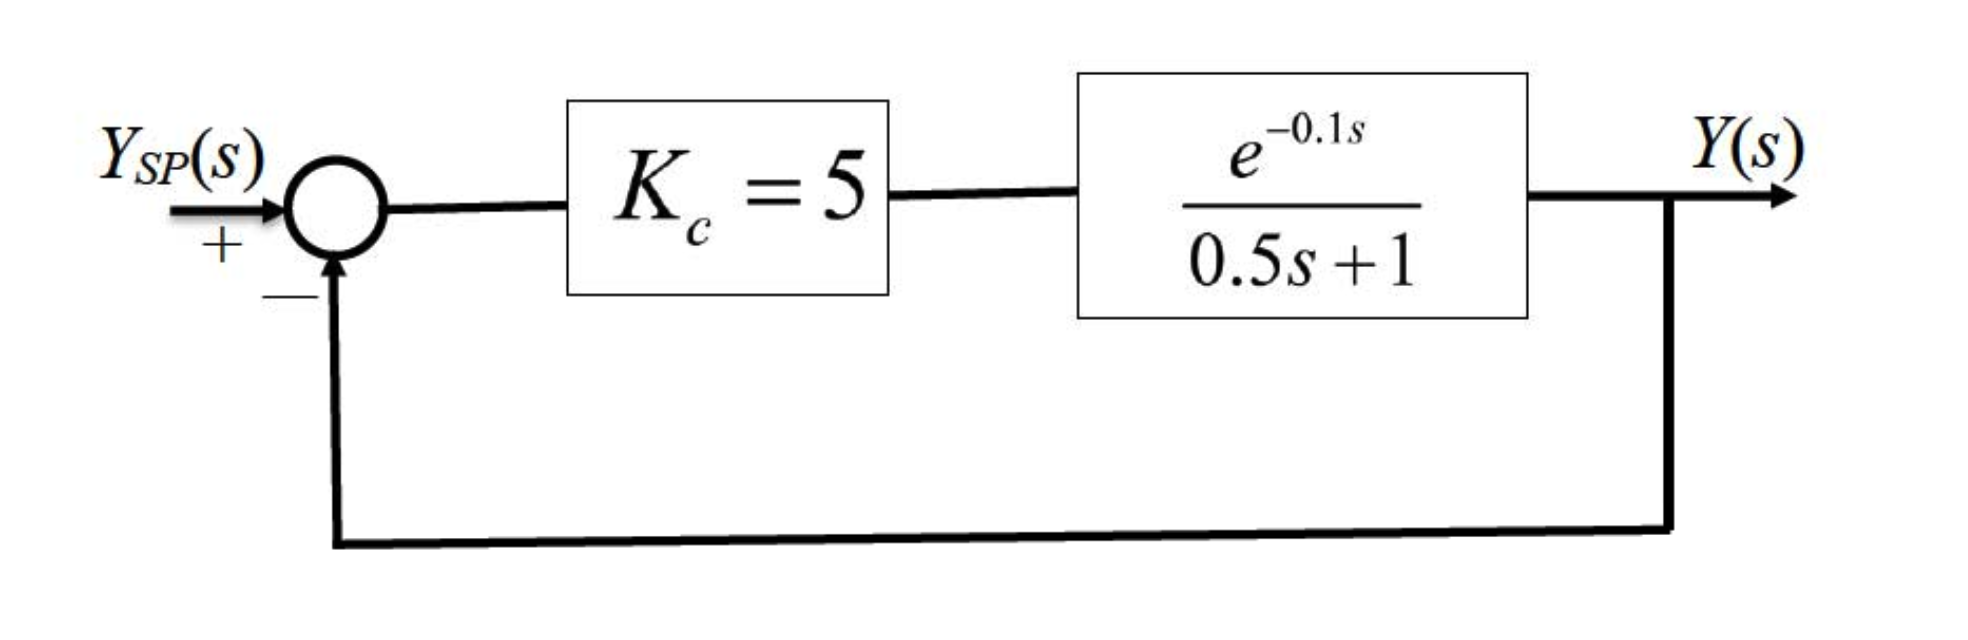
\includegraphics[width=0.5\columnwidth]{Fig/49.png}
        \caption*{}
        \label{fig: 49}
    \end{figure}

    \item Two spherical camphor particles of radii 20 cm and 5 cm, far away from each other, are undergoing sublimation in a stream of air. The mass transfer coefficient is proportional to $1/\sqrt{r\brak{t}}$, where $r\brak{t}$ is the radius of the sphere at time t. Assume that the partial pressure of camphor far away from the surface of the particle is zero. Also, assume quasi-steady state, identical ambient conditions, and negligible heat effects. If $t_1$ $t_2$ are the times required for complete sublimation of the 20 cm and 5 cm camphor particles, respectively, the ratio $t_1/ t_2$ is \rule{2cm}{0.1mm}(rounded off to one decimal place). 
    
\hfill{\brak{\text{GATE CH 2019}}}
    \item A countercurrent absorption tower is designed to remove 95\% of component A from an incoming binary gas mixture using pure solvent B. The mole ratio of A in the inlet gas is 0.02. The carrier gas flow rate is 50 kmol/h. The equilibrium relation is given by Y = 2X, where Y and X are the mole ratios of A in the gas and liquid phases, respectively. If the tower is operated at twice the minimum solvent flow rate, the mole ratio of A in the exit liquid stream is \rule{2cm}{0.1mm} (rounded off to three decimal places). 
    
\hfill{\brak{\text{GATE CH 2019}}}
    \item A binary mixture with components A and B is to be separated in a distillation column to obtain 95 mol\% A as the top product. The binary mixture has a constant relative volatility $\alpha_{AB} = 2$. The column feed is a saturated liquid containing 50 mol\% A. Under the usual simplifying assumptions such as constant molal overflow, negligible heat loss, ideal trays, the minimum reflux ratio for this separation is \rule{2cm}{0.1mm}(rounded off to one decimal place).
    
\hfill{\brak{\text{GATE CH 2019}}}
\newpage
    \item Consider the reactor-separator-recycle process operating under steady state conditions as shown in the figure. The reactor is an ideal Continuous-Stirred Tank Reactor (CSTR), where the reaction $A + B \to C$ occurs. Assume that there is no impurity in the product and recycle streams. Other relevant information are provided in the figure. The mole fraction of $B\brak{x_{B}}$ in the reactor that minimizes the recycle rate is \rule{2cm}{0.1mm}(rounded off to two decimal places). 
    
\hfill{\brak{\text{GATE CH 2019}}}
\begin{figure}[H]
    \centering
    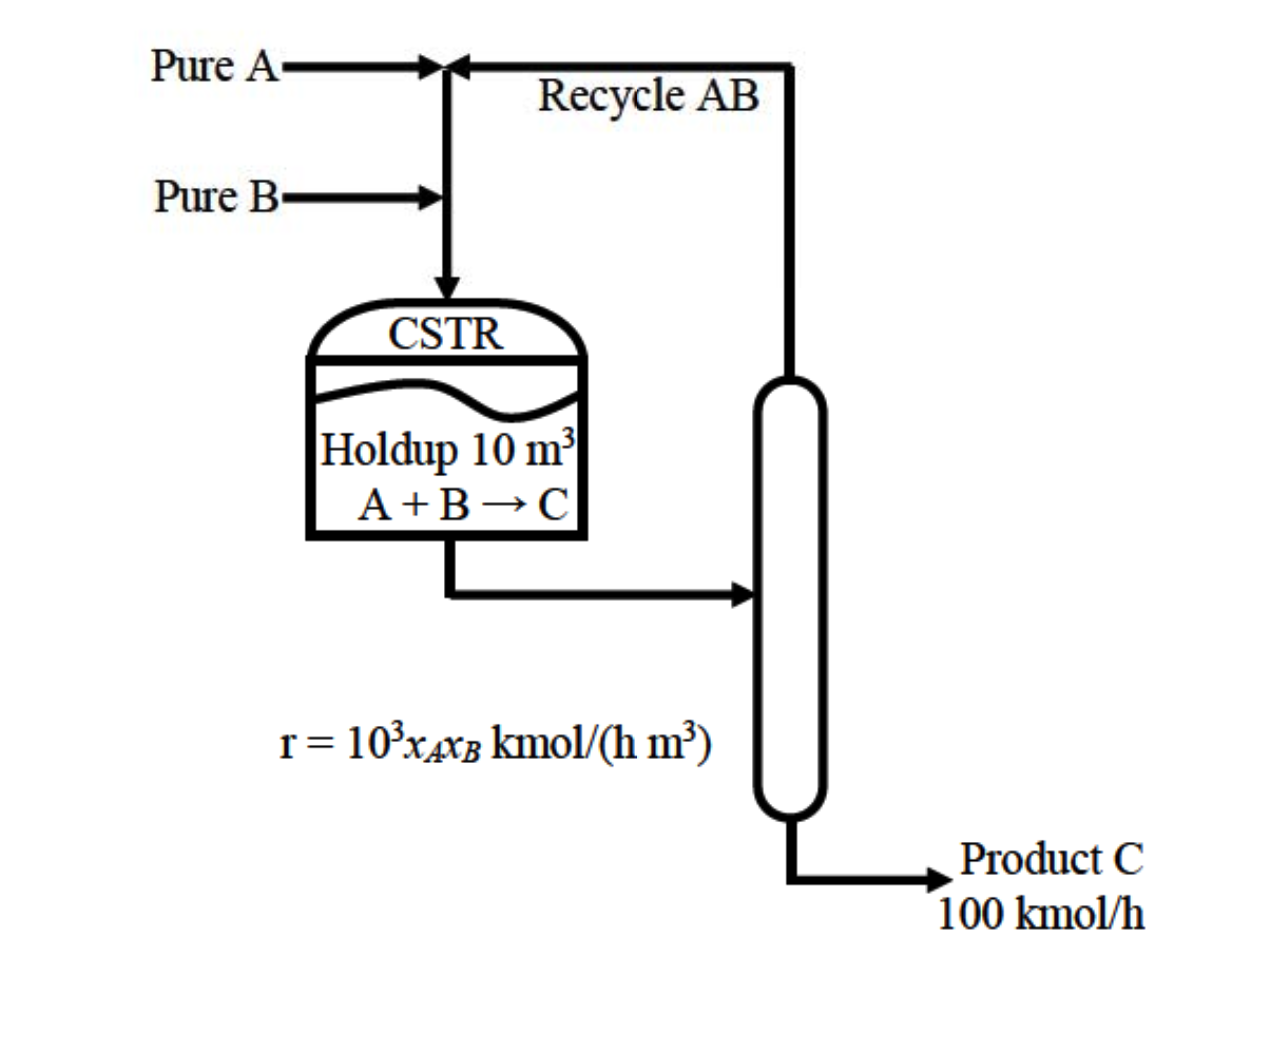
\includegraphics[width=0.5\columnwidth]{Fig/53.png}
    \caption*{}
    \label{fig:Q15}
\end{figure}

    \item Consider two competing equipment A and B. For a compound interest rate of 10\% per annum, in order for equipment B to be the economically cheaper option, its minimum life (in years) is \rule{1cm}{0.1mm}(rounded off to the next higher integer). 
    
\hfill{\brak{\text{GATE CH 2019}}}
    \begin{multicols}{4}
    \begin{enumerate}[label = {}]
      \item Equipment
      \item 
      \item A
      \item B
    \end{enumerate}
\columnbreak
    \begin{enumerate}[label = {}]
        \item Capital Cost
        \item (Rs)
        \item 80,000
        \item 1,60,000
    \end{enumerate}
\columnbreak
    \begin{enumerate}[label = {}]
        \item Yearly Operate
        \item cost(Rs)
        \item 20,000
        \item 15,000
    \end{enumerate}
\columnbreak
    \begin{enumerate}[label = {}]
        \item Equipment Life 
        \item (Years)
        \item 4
        \item ?
    \end{enumerate}
    \end{multicols}

    \item A taxi-car is bought for Rs 10 lakhs. Its salvage value is zero. The expected yearly income after paying all expenses and applicable taxes is Rs 3 lakhs. The compound interest rate is \% per annum. The discounted payback period (in years),is \rule{2cm}{0.1mm}(rounded off to the next higher integer). 
    
\hfill{\brak{\text{GATE CH 2019}}}
\end{enumerate}
    \centering
    \subsection*{END OF QUESTION PAPER}

\end{document}
